\documentclass{article}

\usepackage{amsmath, amssymb}
\usepackage{graphicx}
\usepackage{hyperref}

\begin{document}

\title{Pol Sci 630:  Problem Set 10 Solutions: 2SLS, Matching, Outlier, Heckman}

\author{Prepared by: Anh Le (\href{mailto:anh.le@duke.edu}{anh.le@duke.edu})}

\date{Due Date: Friday, Nov 6, 2015, 12 AM (Beginning of Lab)}

\maketitle

\section{2SLS}

\textbf{\color{red} Insert your comments on the assignment that you are grading above the solution in bold and red text. For example write: "GRADER COMMENT: everything is correct! - 8/8 Points" Also briefly point out which, if any, problems were not solved correctly and what the mistake was. See below for more examples.}

\subsection{Load dataset CigarettesSW from package AER}

\begin{knitrout}
\definecolor{shadecolor}{rgb}{0.969, 0.969, 0.969}\color{fgcolor}\begin{kframe}
\begin{alltt}
\hlkwd{library}\hlstd{(AER)}
\hlkwd{data}\hlstd{(}\hlstr{"CigarettesSW"}\hlstd{)}
\end{alltt}
\end{kframe}
\end{knitrout}

\subsection{Plot the following}

What can we say about the relationship between tax, price, and packs? Note: This is a good way to show the relationship between 3 variables with a 2D plot.

\begin{knitrout}
\definecolor{shadecolor}{rgb}{0.969, 0.969, 0.969}\color{fgcolor}
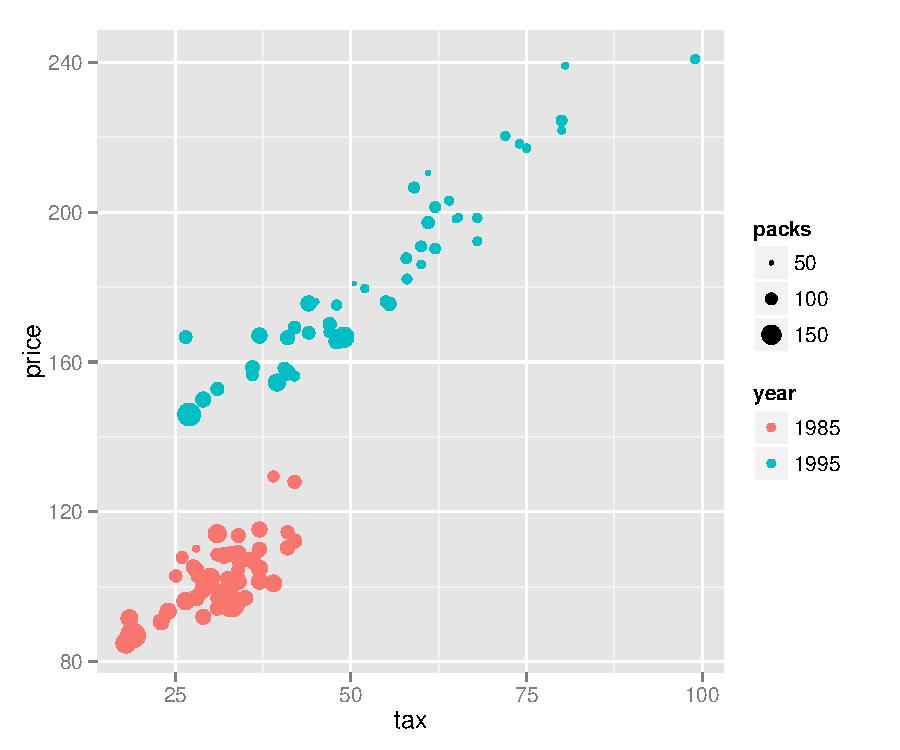
\includegraphics[width=\maxwidth]{figure/unnamed-chunk-2-1} 

\end{knitrout}

\textbf{Solution}

Tax and price are positively correlated. This gives a hint that tax can be a good instrument for price.

Tax and price are negatively correlated with the number of cigarette packs consumed per capita.

\subsection{Divide variable income by 1000 (for interpretability)}

\begin{knitrout}
\definecolor{shadecolor}{rgb}{0.969, 0.969, 0.969}\color{fgcolor}\begin{kframe}
\begin{alltt}
\hlstd{CigarettesSW}\hlopt{$}\hlstd{income} \hlkwb{<-} \hlstd{CigarettesSW}\hlopt{$}\hlstd{income} \hlopt{/} \hlnum{1000}
\end{alltt}
\end{kframe}
\end{knitrout}


\subsection{Run 2SLS}

Run 2SLS with \verb`ivreg`. Outcome: packs. Exogenous var: income. Endogenous var: price, whose instrument is tax. Interpret the coefficient of \verb`income` and \verb`price`.

\textbf{Solution}

\begin{kframe}
\begin{alltt}
\hlkwd{library}\hlstd{(stargazer)}
\hlstd{m11} \hlkwb{<-} \hlkwd{ivreg}\hlstd{(packs} \hlopt{~} \hlstd{income} \hlopt{+} \hlstd{price} \hlopt{|} \hlstd{income} \hlopt{+} \hlstd{tax,} \hlkwc{data} \hlstd{= CigarettesSW)}
\hlkwd{stargazer}\hlstd{(m11)}
\end{alltt}
\end{kframe}
% Table created by stargazer v.5.2 by Marek Hlavac, Harvard University. E-mail: hlavac at fas.harvard.edu
% Date and time: Fri, Nov 18, 2016 - 05:10:26 PM
\begin{table}[!htbp] \centering 
  \caption{} 
  \label{} 
\begin{tabular}{@{\extracolsep{5pt}}lc} 
\\[-1.8ex]\hline 
\hline \\[-1.8ex] 
 & \multicolumn{1}{c}{\textit{Dependent variable:}} \\ 
\cline{2-2} 
\\[-1.8ex] & packs \\ 
\hline \\[-1.8ex] 
 income & $-$0.00002 \\ 
  & (0.00002) \\ 
  & \\ 
 price & $-$0.398$^{***}$ \\ 
  & (0.055) \\ 
  & \\ 
 Constant & 168.488$^{***}$ \\ 
  & (7.673) \\ 
  & \\ 
\hline \\[-1.8ex] 
Observations & 96 \\ 
R$^{2}$ & 0.436 \\ 
Adjusted R$^{2}$ & 0.424 \\ 
Residual Std. Error & 19.637 (df = 93) \\ 
\hline 
\hline \\[-1.8ex] 
\textit{Note:}  & \multicolumn{1}{r}{$^{*}$p$<$0.1; $^{**}$p$<$0.05; $^{***}$p$<$0.01} \\ 
\end{tabular} 
\end{table} 


1000 dollar increase in income leads to \ensuremath{-2.2311969\times 10^{-5}} change in number of packs per capita, but the effect is not significant.

1 dollar increase in price leads to \ensuremath{-0.3978933} change in number of packs per capita, holding other constants. The coefficient is statistically significant.

\subsection{2SLS diagnostics: use F-test to check for weak instrument}

\textbf{Solution}

\begin{knitrout}
\definecolor{shadecolor}{rgb}{0.969, 0.969, 0.969}\color{fgcolor}\begin{kframe}
\begin{alltt}
\hlkwd{summary}\hlstd{(m11,} \hlkwc{diagnostics} \hlstd{=} \hlnum{TRUE}\hlstd{)}
\end{alltt}
\begin{verbatim}
## 
## Call:
## ivreg(formula = packs ~ income + price | income + tax, data = CigarettesSW)
## 
## Residuals:
##       Min        1Q    Median        3Q       Max 
## -56.16120 -10.40243   0.07866   6.87649  67.85671 
## 
## Coefficients:
##               Estimate Std. Error t value Pr(>|t|)    
## (Intercept)  1.685e+02  7.673e+00  21.957  < 2e-16 ***
## income      -2.231e-05  1.803e-05  -1.238    0.219    
## price       -3.979e-01  5.502e-02  -7.232 1.31e-10 ***
## 
## Diagnostic tests:
##                  df1 df2 statistic p-value    
## Weak instruments   1  93   341.145  <2e-16 ***
## Wu-Hausman         1  92     2.312   0.132    
## Sargan             0  NA        NA      NA    
## ---
## Signif. codes:  0 '***' 0.001 '**' 0.01 '*' 0.05 '.' 0.1 ' ' 1
## 
## Residual standard error: 19.64 on 93 degrees of freedom
## Multiple R-Squared: 0.436,	Adjusted R-squared: 0.4239 
## Wald test: 35.23 on 2 and 93 DF,  p-value: 4.081e-12
\end{verbatim}
\end{kframe}
\end{knitrout}

The weak instrument test (i.e. F-test) rejects the null hypothesis that the instrument is not correlated with the endogenous variable (p-value = \ensuremath{7.1137017\times 10^{-33}}). So our instruments are not weak.

\subsection{2SLS by hand}

Run the 2SLS by hand, i.e. not using \verb`ivreg`, but run 2 stages of \verb`lm`. Do you get the same estimate and F-statistic from \verb`ivreg`?

\textbf{Solution}

\begin{kframe}
\begin{alltt}
\hlstd{m_stage1} \hlkwb{<-} \hlkwd{lm}\hlstd{(price} \hlopt{~} \hlstd{tax} \hlopt{+} \hlstd{income,} \hlkwc{data} \hlstd{= CigarettesSW)}
\hlstd{CigarettesSW}\hlopt{$}\hlstd{price_hat} \hlkwb{<-} \hlkwd{predict}\hlstd{(m_stage1)}

\hlstd{m_stage2} \hlkwb{<-} \hlkwd{lm}\hlstd{(packs} \hlopt{~} \hlstd{income} \hlopt{+} \hlstd{price_hat,} \hlkwc{data} \hlstd{= CigarettesSW)}
\hlkwd{stargazer}\hlstd{(m_stage2)}
\end{alltt}
\end{kframe}
% Table created by stargazer v.5.2 by Marek Hlavac, Harvard University. E-mail: hlavac at fas.harvard.edu
% Date and time: Fri, Nov 18, 2016 - 05:10:27 PM
\begin{table}[!htbp] \centering 
  \caption{} 
  \label{} 
\begin{tabular}{@{\extracolsep{5pt}}lc} 
\\[-1.8ex]\hline 
\hline \\[-1.8ex] 
 & \multicolumn{1}{c}{\textit{Dependent variable:}} \\ 
\cline{2-2} 
\\[-1.8ex] & packs \\ 
\hline \\[-1.8ex] 
 income & $-$0.00002 \\ 
  & (0.00002) \\ 
  & \\ 
 price\_hat & $-$0.398$^{***}$ \\ 
  & (0.055) \\ 
  & \\ 
 Constant & 168.488$^{***}$ \\ 
  & (7.733) \\ 
  & \\ 
\hline \\[-1.8ex] 
Observations & 96 \\ 
R$^{2}$ & 0.427 \\ 
Adjusted R$^{2}$ & 0.415 \\ 
Residual Std. Error & 19.788 (df = 93) \\ 
F Statistic & 34.693$^{***}$ (df = 2; 93) \\ 
\hline 
\hline \\[-1.8ex] 
\textit{Note:}  & \multicolumn{1}{r}{$^{*}$p$<$0.1; $^{**}$p$<$0.05; $^{***}$p$<$0.01} \\ 
\end{tabular} 
\end{table} 


The coefficients are exactly the same (by hand: \ensuremath{-0.3978933}, by ivreg: \ensuremath{-0.3978933}).

The F-statistic is also the same (by hand: 198.4830451, by ivreg: 341.1446676)

\section{Matching}

\subsection{Load dataset lalonde from MatchIt, show covariate imbalance}

Plot the following. Hint: Look up \verb|position="dodge"| for ggplot2

\begin{knitrout}
\definecolor{shadecolor}{rgb}{0.969, 0.969, 0.969}\color{fgcolor}\begin{kframe}
\begin{alltt}
\hlkwd{library}\hlstd{(MatchIt)}
\end{alltt}


{\ttfamily\noindent\bfseries\color{errorcolor}{\#\# Error in library(MatchIt): there is no package called 'MatchIt'}}\begin{alltt}
\hlkwd{data}\hlstd{(}\hlstr{"lalonde"}\hlstd{)}
\end{alltt}


{\ttfamily\noindent\color{warningcolor}{\#\# Warning in data("{}lalonde"{}): data set 'lalonde' not found}}\begin{alltt}
\hlkwd{ggplot}\hlstd{(}\hlkwc{data} \hlstd{= lalonde)} \hlopt{+}
  \hlkwd{geom_histogram}\hlstd{(}\hlkwd{aes}\hlstd{(}\hlkwc{x} \hlstd{= black,} \hlkwc{fill} \hlstd{=} \hlkwd{factor}\hlstd{(treat)),}
                 \hlkwc{position} \hlstd{=} \hlstr{"dodge"}\hlstd{)}
\end{alltt}


{\ttfamily\noindent\bfseries\color{errorcolor}{\#\# Error in ggplot(data = lalonde): object 'lalonde' not found}}\end{kframe}
\end{knitrout}

\subsection{See the effect of omitting an important variable}

Regress re78 against 1) treat, age, educ; 2) treat, age, educ, black. Do the treatment effect differ a lot? Why?

\textbf{Solution}

\begin{knitrout}
\definecolor{shadecolor}{rgb}{0.969, 0.969, 0.969}\color{fgcolor}\begin{kframe}
\begin{alltt}
\hlkwd{lm}\hlstd{(re78} \hlopt{~} \hlstd{treat} \hlopt{+} \hlstd{age} \hlopt{+} \hlstd{educ,} \hlkwc{data} \hlstd{= lalonde)}
\end{alltt}


{\ttfamily\noindent\bfseries\color{errorcolor}{\#\# Error in is.data.frame(data): object 'lalonde' not found}}\begin{alltt}
\hlkwd{lm}\hlstd{(re78} \hlopt{~} \hlstd{treat} \hlopt{+} \hlstd{age} \hlopt{+} \hlstd{educ} \hlopt{+} \hlstd{black,} \hlkwc{data} \hlstd{= lalonde)}
\end{alltt}


{\ttfamily\noindent\bfseries\color{errorcolor}{\#\# Error in is.data.frame(data): object 'lalonde' not found}}\end{kframe}
\end{knitrout}

If we do not control for \verb`black`, we would wrongly conclude that the treatment effect is negative. This is because we have a lot of blacks in the treatment group, and blacks tend to have poorer outcomes.

\subsection{Running CEM: Matching and check balance}

Match the treatment and the control group based on age, educ, and black. Check the balance

\textbf{Solution}

\begin{knitrout}
\definecolor{shadecolor}{rgb}{0.969, 0.969, 0.969}\color{fgcolor}\begin{kframe}
\begin{alltt}
\hlstd{m.out} \hlkwb{<-} \hlkwd{matchit}\hlstd{(treat} \hlopt{~} \hlstd{age} \hlopt{+} \hlstd{educ} \hlopt{+} \hlstd{black,} \hlkwc{data} \hlstd{= lalonde,}
                 \hlkwc{method} \hlstd{=} \hlstr{"cem"}\hlstd{)}
\end{alltt}


{\ttfamily\noindent\bfseries\color{errorcolor}{\#\# Error in eval(expr, envir, enclos): could not find function "{}matchit"{}}}\begin{alltt}
\hlkwd{summary}\hlstd{(m.out)} \hlcom{# to check balance}
\end{alltt}


{\ttfamily\noindent\bfseries\color{errorcolor}{\#\# Error in summary(m.out): object 'm.out' not found}}\end{kframe}
\end{knitrout}

We get exact balance after running CEM.

\subsection{Running CEM: Analysis after matching}

Run a weighted regression of re78 against 1) treat, age, educ, 2) treat, age, educ, and black. Do the treatment effect differ? Compare this result with part 2.

\textbf{Solution}

\begin{knitrout}
\definecolor{shadecolor}{rgb}{0.969, 0.969, 0.969}\color{fgcolor}\begin{kframe}
\begin{alltt}
\hlcom{# Get the matched data}
\hlstd{lalonde_matched} \hlkwb{<-} \hlkwd{match.data}\hlstd{(m.out)}
\end{alltt}


{\ttfamily\noindent\bfseries\color{errorcolor}{\#\# Error in eval(expr, envir, enclos): could not find function "{}match.data"{}}}\begin{alltt}
\hlcom{# Run weighted regression to get the causal treatment effect}
\hlkwd{lm}\hlstd{(re78} \hlopt{~} \hlstd{treat} \hlopt{+} \hlstd{age} \hlopt{+} \hlstd{educ,}
   \hlkwc{data} \hlstd{= lalonde_matched,} \hlkwc{weights} \hlstd{= lalonde_matched}\hlopt{$}\hlstd{weights)}
\end{alltt}


{\ttfamily\noindent\bfseries\color{errorcolor}{\#\# Error in is.data.frame(data): object 'lalonde\_matched' not found}}\begin{alltt}
\hlkwd{lm}\hlstd{(re78} \hlopt{~} \hlstd{treat} \hlopt{+} \hlstd{age} \hlopt{+} \hlstd{educ} \hlopt{+} \hlstd{black,}
   \hlkwc{data} \hlstd{= lalonde_matched,} \hlkwc{weights} \hlstd{= lalonde_matched}\hlopt{$}\hlstd{weights)}
\end{alltt}


{\ttfamily\noindent\bfseries\color{errorcolor}{\#\# Error in is.data.frame(data): object 'lalonde\_matched' not found}}\end{kframe}
\end{knitrout}

The treatment effect doen't differ by a lot across the two regressions. It's because in the matched data, we have equal number of blacks in the control and the treatment group.

\section{Heckman}

\subsection{Load Mroz87 data from package sampleSelection}

\begin{knitrout}
\definecolor{shadecolor}{rgb}{0.969, 0.969, 0.969}\color{fgcolor}\begin{kframe}
\begin{alltt}
\hlkwd{library}\hlstd{(sampleSelection)}
\end{alltt}


{\ttfamily\noindent\bfseries\color{errorcolor}{\#\# Error in library(sampleSelection): there is no package called 'sampleSelection'}}\begin{alltt}
\hlkwd{data}\hlstd{(Mroz87)}
\end{alltt}


{\ttfamily\noindent\color{warningcolor}{\#\# Warning in data(Mroz87): data set 'Mroz87' not found}}\end{kframe}
\end{knitrout}

\subsection{Run a Heckman model}

The selection variable is lfp. Run a heckman model with huswage, kid5, educ, city explaning the selection, and educ and city explaning the outcome variable log(wage). Interpret the result for the outcome model

\textbf{Solution}

\begin{knitrout}
\definecolor{shadecolor}{rgb}{0.969, 0.969, 0.969}\color{fgcolor}\begin{kframe}
\begin{alltt}
\hlstd{a} \hlkwb{<-} \hlkwd{heckit}\hlstd{(lfp} \hlopt{~} \hlstd{huswage} \hlopt{+} \hlstd{kids5} \hlopt{+} \hlstd{educ} \hlopt{+} \hlstd{city,} \hlkwd{log}\hlstd{(wage)} \hlopt{~} \hlstd{educ} \hlopt{+} \hlstd{city,} \hlkwc{data}\hlstd{=Mroz87)}
\end{alltt}


{\ttfamily\noindent\bfseries\color{errorcolor}{\#\# Error in eval(expr, envir, enclos): could not find function "{}heckit"{}}}\begin{alltt}
\hlkwd{summary}\hlstd{(a)}
\end{alltt}


{\ttfamily\noindent\bfseries\color{errorcolor}{\#\# Error in summary(a): object 'a' not found}}\end{kframe}
\end{knitrout}





